% Od tego momentu porównujemy algorytmy między sobą
\section{Zastosowania}

\subsection{Uwierzytelnianie}
\begin{frame}{Uwierzytelnianie}
    \begin{itemize}
        \pause
        \item Podpisy cyfrowe
        \pause
        \item Certifikaty
    \end{itemize}
\end{frame}

\begin{frame}{Podpisy cyfrowe - charakterystyka}
\pause
    \begin{itemize}
        \item Uwierzytelnianie nadawcy
        \pause
        \item Integralność danych
        \pause
        \item Niezaprzeczalność
    \end{itemize}
    
\end{frame}

\begin{frame}{Podpisy cyfrowe - metoda działania}
    \begin{columns}
        \column{0.5\textwidth}
        \textbf{RSA}
        \begin{itemize}
            \item Hashowanie wiadomości
            \item Szyfrowanie hashu kluczem prywatnym
            \item Odszyfrowanie hashu kluczem publicznym
            \item Porównanie hashy
        \end{itemize}

        \column{0.5\textwidth}
        \textbf{ECC (ECDSA)}
        \begin{itemize}
            \item Hashowanie wiadomości
            \item Generowanie losowej wartości $k$
            \item Obliczenie $(r, s)$
            \item Porównanie podpisu
        \end{itemize}
        \vspace{6pt}
    \end{columns}
\end{frame}

\begin{frame}{Certifikaty - budowa}
    \begin{itemize}
        \item Dane o właścicielu
        \item Klucz publiczny
        \item Podpis cyfrowy
        \item Okres ważności
        \item Algorytm podpisu
    \end{itemize}

\end{frame}

\begin{frame}{Certifikaty - działanie}
    \begin{itemize}
        \item Wysłanie certyfikatu do serwera
        \item Serwer sprawdza ważność i poprawność certyfikatu
        \item Po pozytywnej weryfikacji serwer szyfruje sesję i kontynuuje komunikację
    \end{itemize}
    
\end{frame}

\begin{frame}{Certyfikaty - algorytmy}

    \begin{columns}
        \column{0.5\textwidth}
        \centering
        
        \textbf{RSA}
        \begin{itemize}
            \item Powszechnie stosowany historycznie
            \item Większe klucze $\rightarrow$ większe wymagania sprzętowe
        \end{itemize}
        
        \column{0.5\textwidth}
        \centering

        \textbf{ECC}  
        \begin{itemize}
            \item Coraz popularniejszy
            \item Krótsze klucze $\rightarrow$ mniejsze wymagania sprzętowe
        \end{itemize}
        \vspace{7.5pt}

    \end{columns}

\end{frame}


\subsection{}
\begin{frame}{Kryptowaluty}
\begin{center}
    \begin{tabular}{cc}
        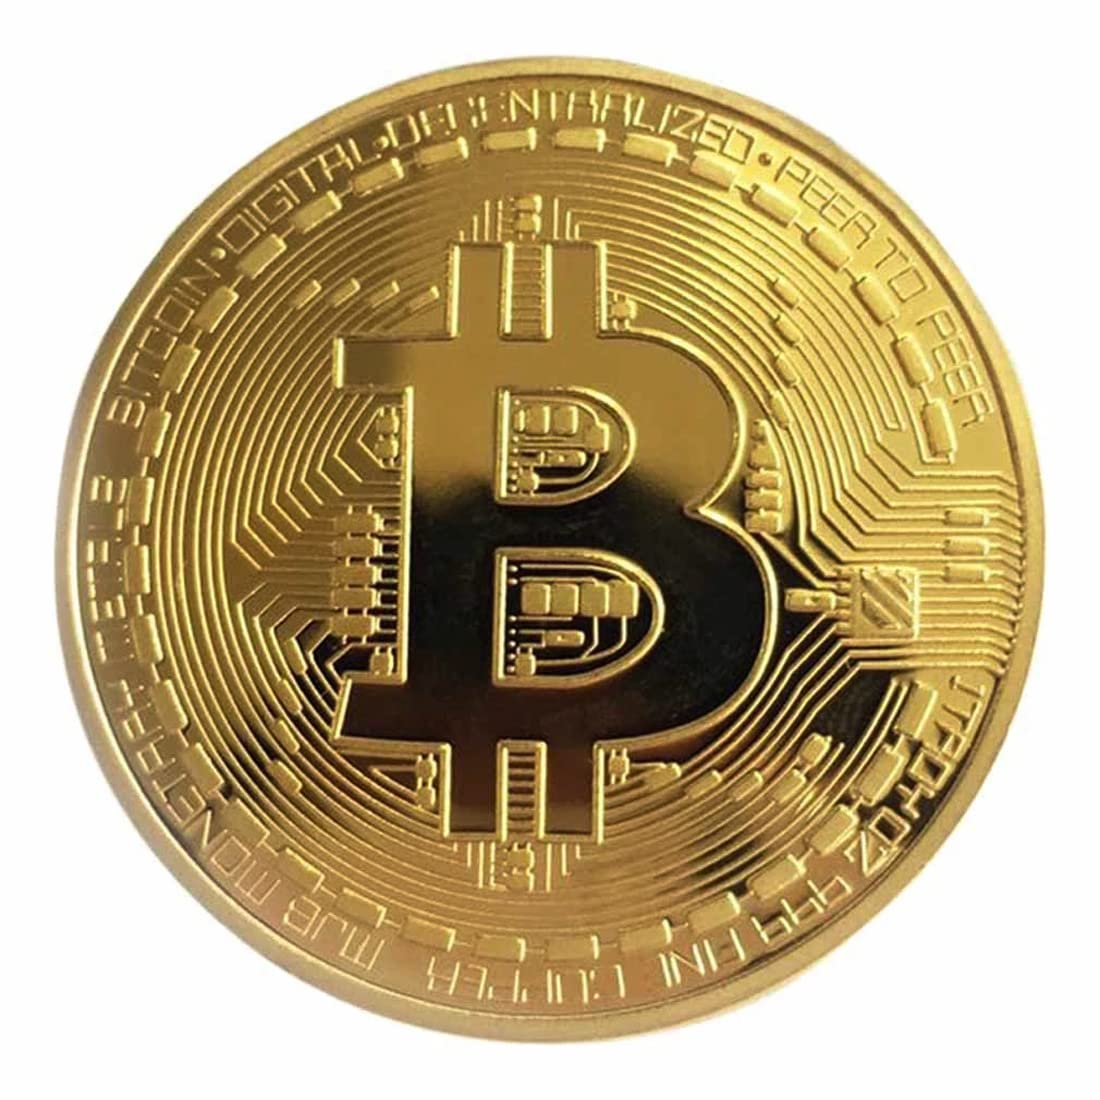
\includegraphics[width=0.3\textwidth, height=0.3\textwidth ]{applications/graphics/Bitcoin.jpg} & 
\includegraphics[width=0.3\textwidth, height=0.3\textwidth]{applications/graphics/Ethereum.png} \\
        
\includegraphics[width=0.3\textwidth, height=0.3\textwidth]{applications/graphics/Dogecoin.png} & 
\includegraphics[width=0.3\textwidth, height=0.3\textwidth]{applications/graphics/Litecoin.jpg} \\
    \end{tabular}
\end{center}
    
\end{frame}

\begin{frame}{Komunikatory E2E - metoda działania}
    \begin{itemize}
        \item Wiadomości są widoczne tylko dla nadawcy i odbiorcy
        \item Klucz publiczny jest przesyłany do serwera
        \item Serwer przesyła klucz publiczny do odbiorcy
        \item Odbiorca odszyfrowuje wiadomość kluczem prywatnym
    \end{itemize}
\end{frame}
\begin{frame}{Komunikatory E2E - przykłady}
    \begin{center}
        \begin{minipage}{0.1\textwidth}
            
\includegraphics[width=\textwidth]{applications/graphics/Signal.png}
        \end{minipage}
        \begin{minipage}{0.6\textwidth}
            \textbf{X3DH oraz Curve25519}
        \end{minipage}

        \vspace{0.3cm}

        \begin{minipage}{0.1\textwidth}
            
\includegraphics[width=\textwidth]{applications/graphics/WhatsApp.png}
        \end{minipage}
        \begin{minipage}{0.6\textwidth}
            \textbf{Curve25519}
        \end{minipage}

        \vspace{0.3cm}

        \begin{minipage}{0.1\textwidth}
            
\includegraphics[width=\textwidth]{applications/graphics/Messenger.png}
        \end{minipage}
        \begin{minipage}{0.6\textwidth}
            \textbf{Signal Protocol}
        \end{minipage}

        \vspace{0.3cm}

        \begin{minipage}{0.1\textwidth}
            
\includegraphics[width=\textwidth]{applications/graphics/Imessage.png}
        \end{minipage}
        \begin{minipage}{0.6\textwidth}
            \textbf{RSA-2048 oraz ECDSA/ECDH}
        \end{minipage}
    \end{center}
\end{frame}

\begin{frame}{IoT}
    \begin{itemize}
        \item Uwierzytelnianie urządzeń (RSA/ECC)
        \item Szyfrowanie komunikacji (TLS, MQTT-TLS)
        \item Bezpieczne aktualizacje OTA
    \end{itemize}
\end{frame}
